\section{Результаты измерений}
\subsection{Дифракция Френеля}
Ширина щели $S_{2}$ $b = 0{,}171 \pm 0{,}0005\;\text{мм}$, $\lambda = 546{,}1\;\text{нм}$.

\begin{tabular}{|l|l|l|l|}
\hline
$n$ & $x,\pm 0{,}5\;\text{мм}$ & $x_{n} - x_{0}, \pm 0{,}1\;\text{мм}$ & $2\xi,\;\text{мм}$ \\\hline
   $0$ & $409{,}0$ & $0$ & $0$ \\\hline
    $1$ & $422{,}0$ & $13{,}0$ & $0{,}17 \pm 0{,}01$ \\\hline
    $2$ & $416{,}0$ & $7{,}0$ & $0{,}17 \pm 0{,}01$ \\\hline
    $3$ & $414{,}0$ & $5{,}0$ & $0{,}18 \pm 0{,}02$ \\\hline
    $4$ & $412{,}0$ & $3{,}0$ & $0{,}16 \pm 0{,}02$ \\\hline
\end{tabular}

\begin{figure}[ht!]
    \center{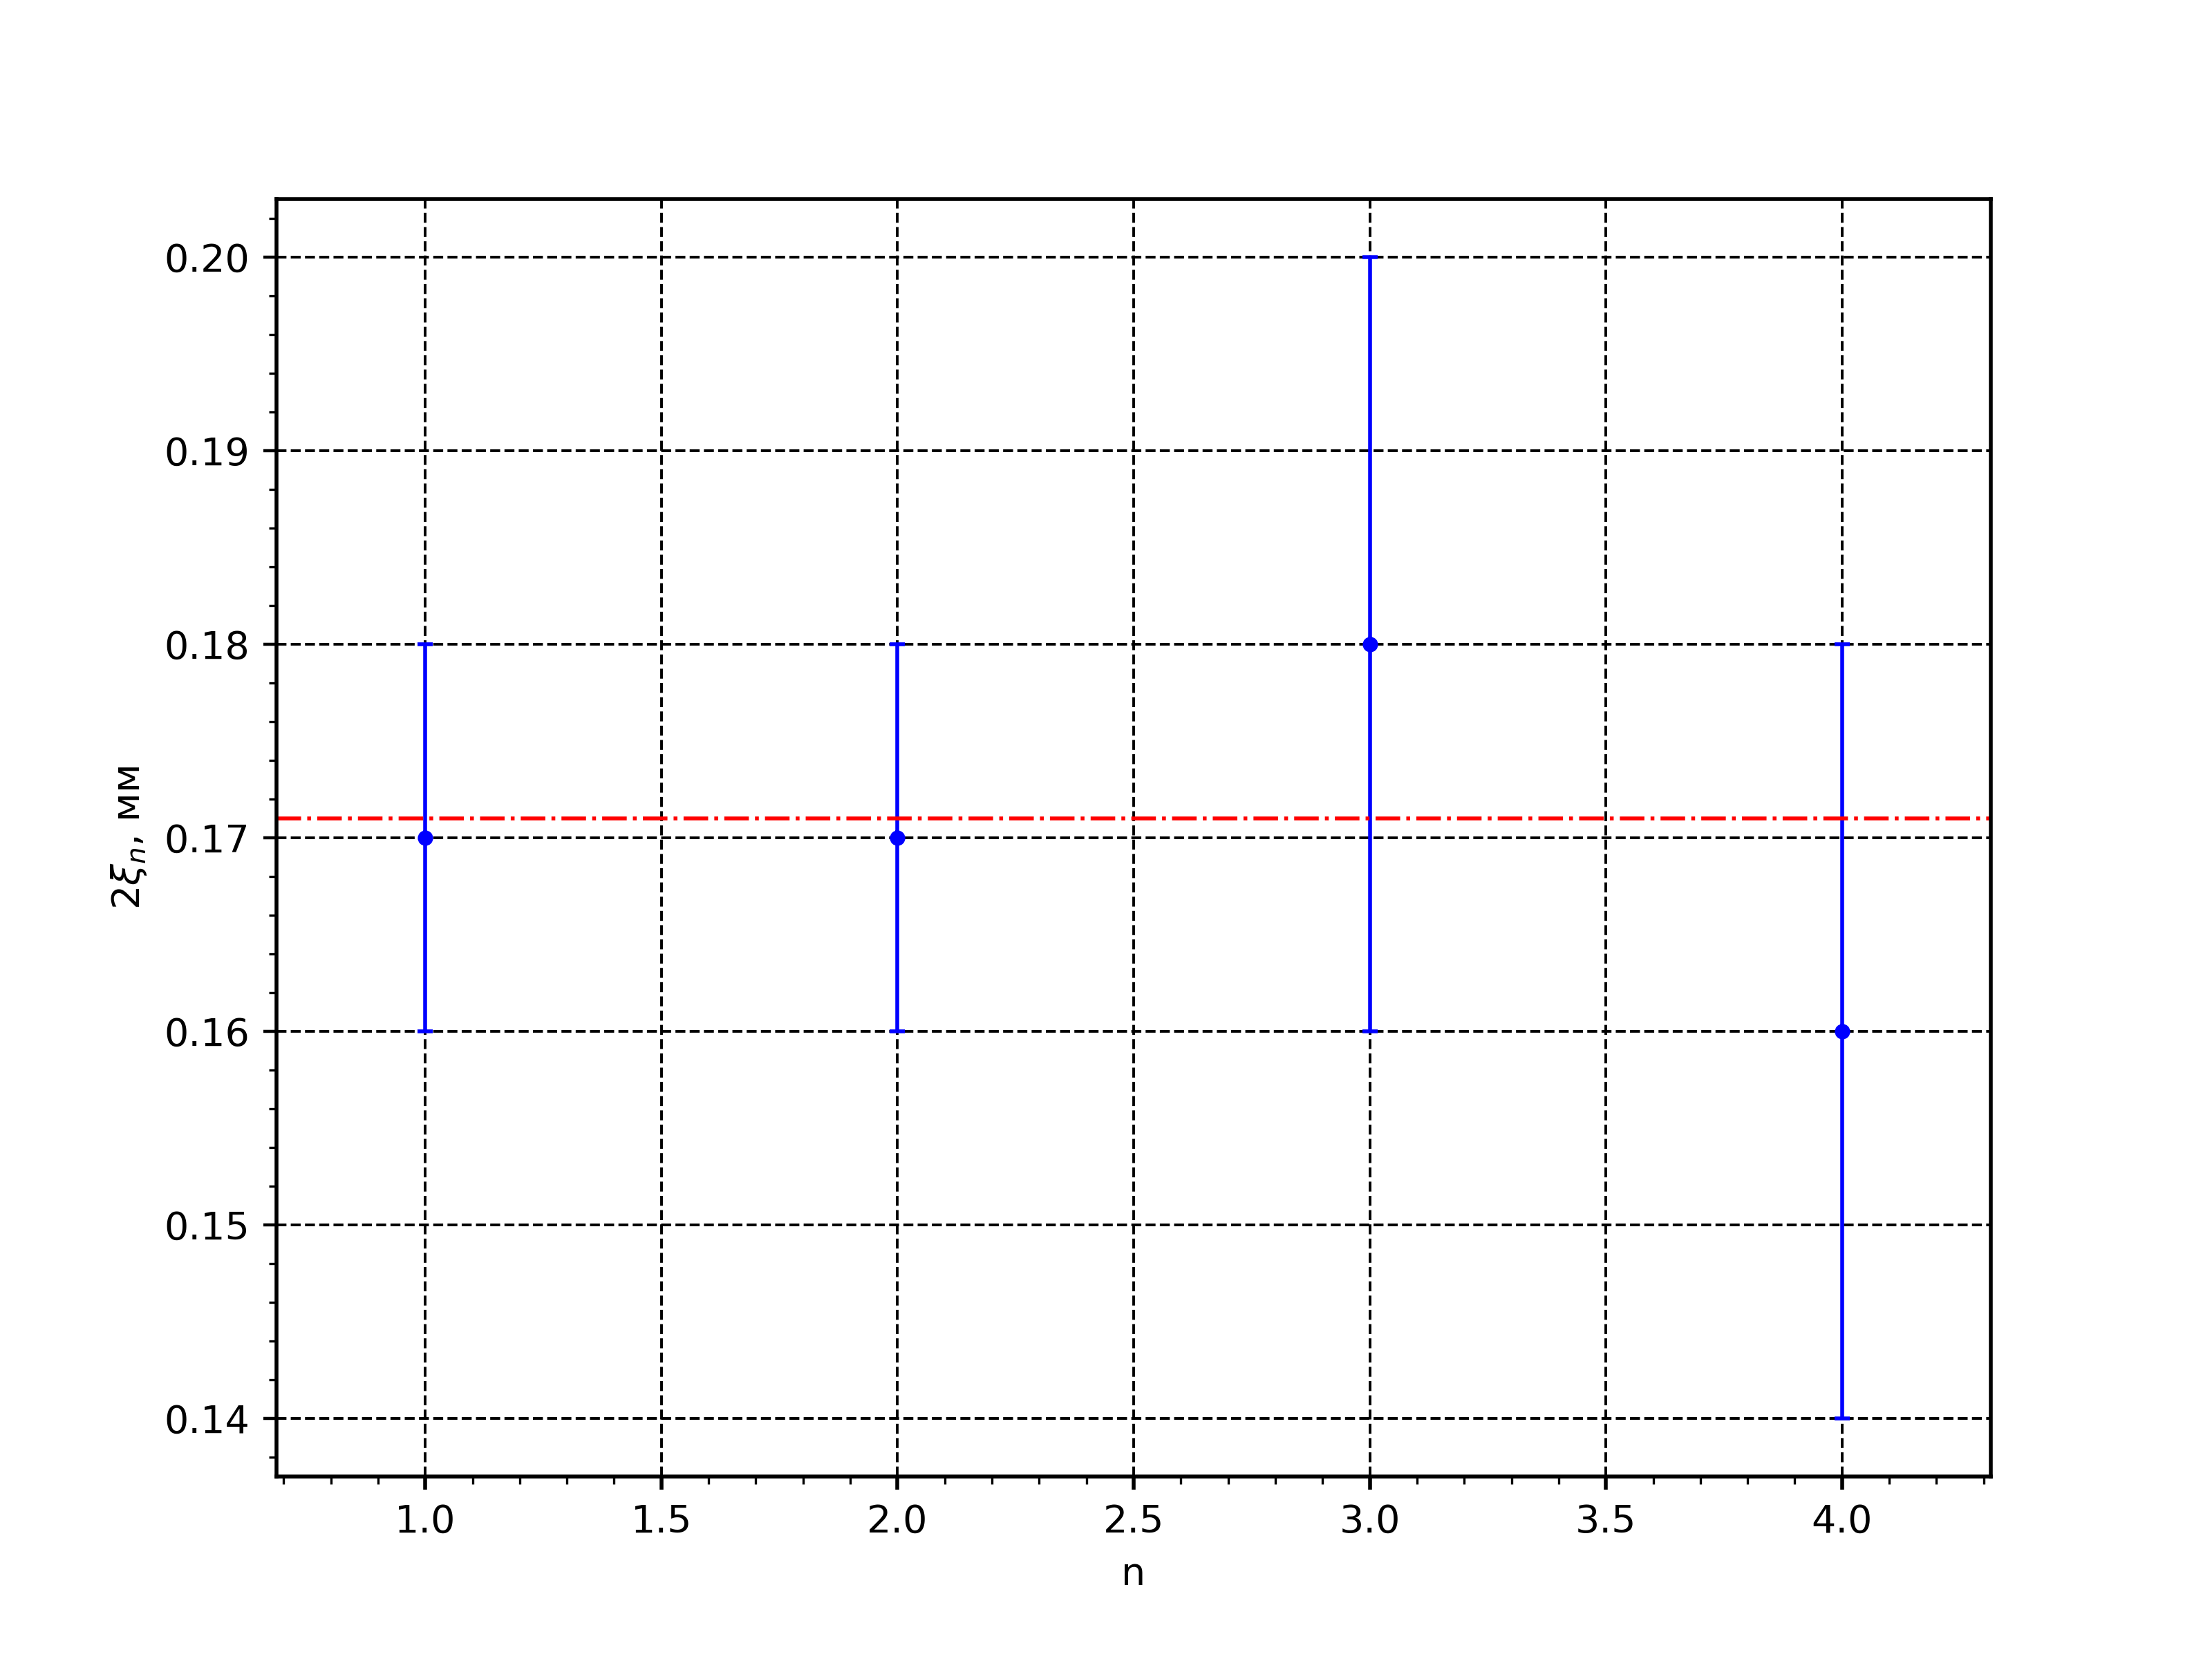
\includegraphics[width=0.8\linewidth]{../img/plota.png}}
\end{figure}

\subsection{Дифракция Фраунгофера на щели}
$b = 0{,}3975 \pm 0{,}0005\;\text{мм}$, $f = 12{,}8\;\text{см}$. 

\begin{tabular}{|l|l|l|l|l|l|l|l|l|l|}
\hline
    $n$ & -4 & -3 & -2 & -1 & 0 & 1 & 2 & 3 & 5 \\\hline
    $x,\pm\;0{,}1];\text{мм}$ & $2{,}2$ & $2{,}4$ & $2{,}6$ & $2{,}8$ & $3{,}0$ & $3{,}2$ & $3{,}4$ & $3{,}6$ & $3{,}8$ \\\hline
\end{tabular}
\begin{figure}[ht!]
    \center{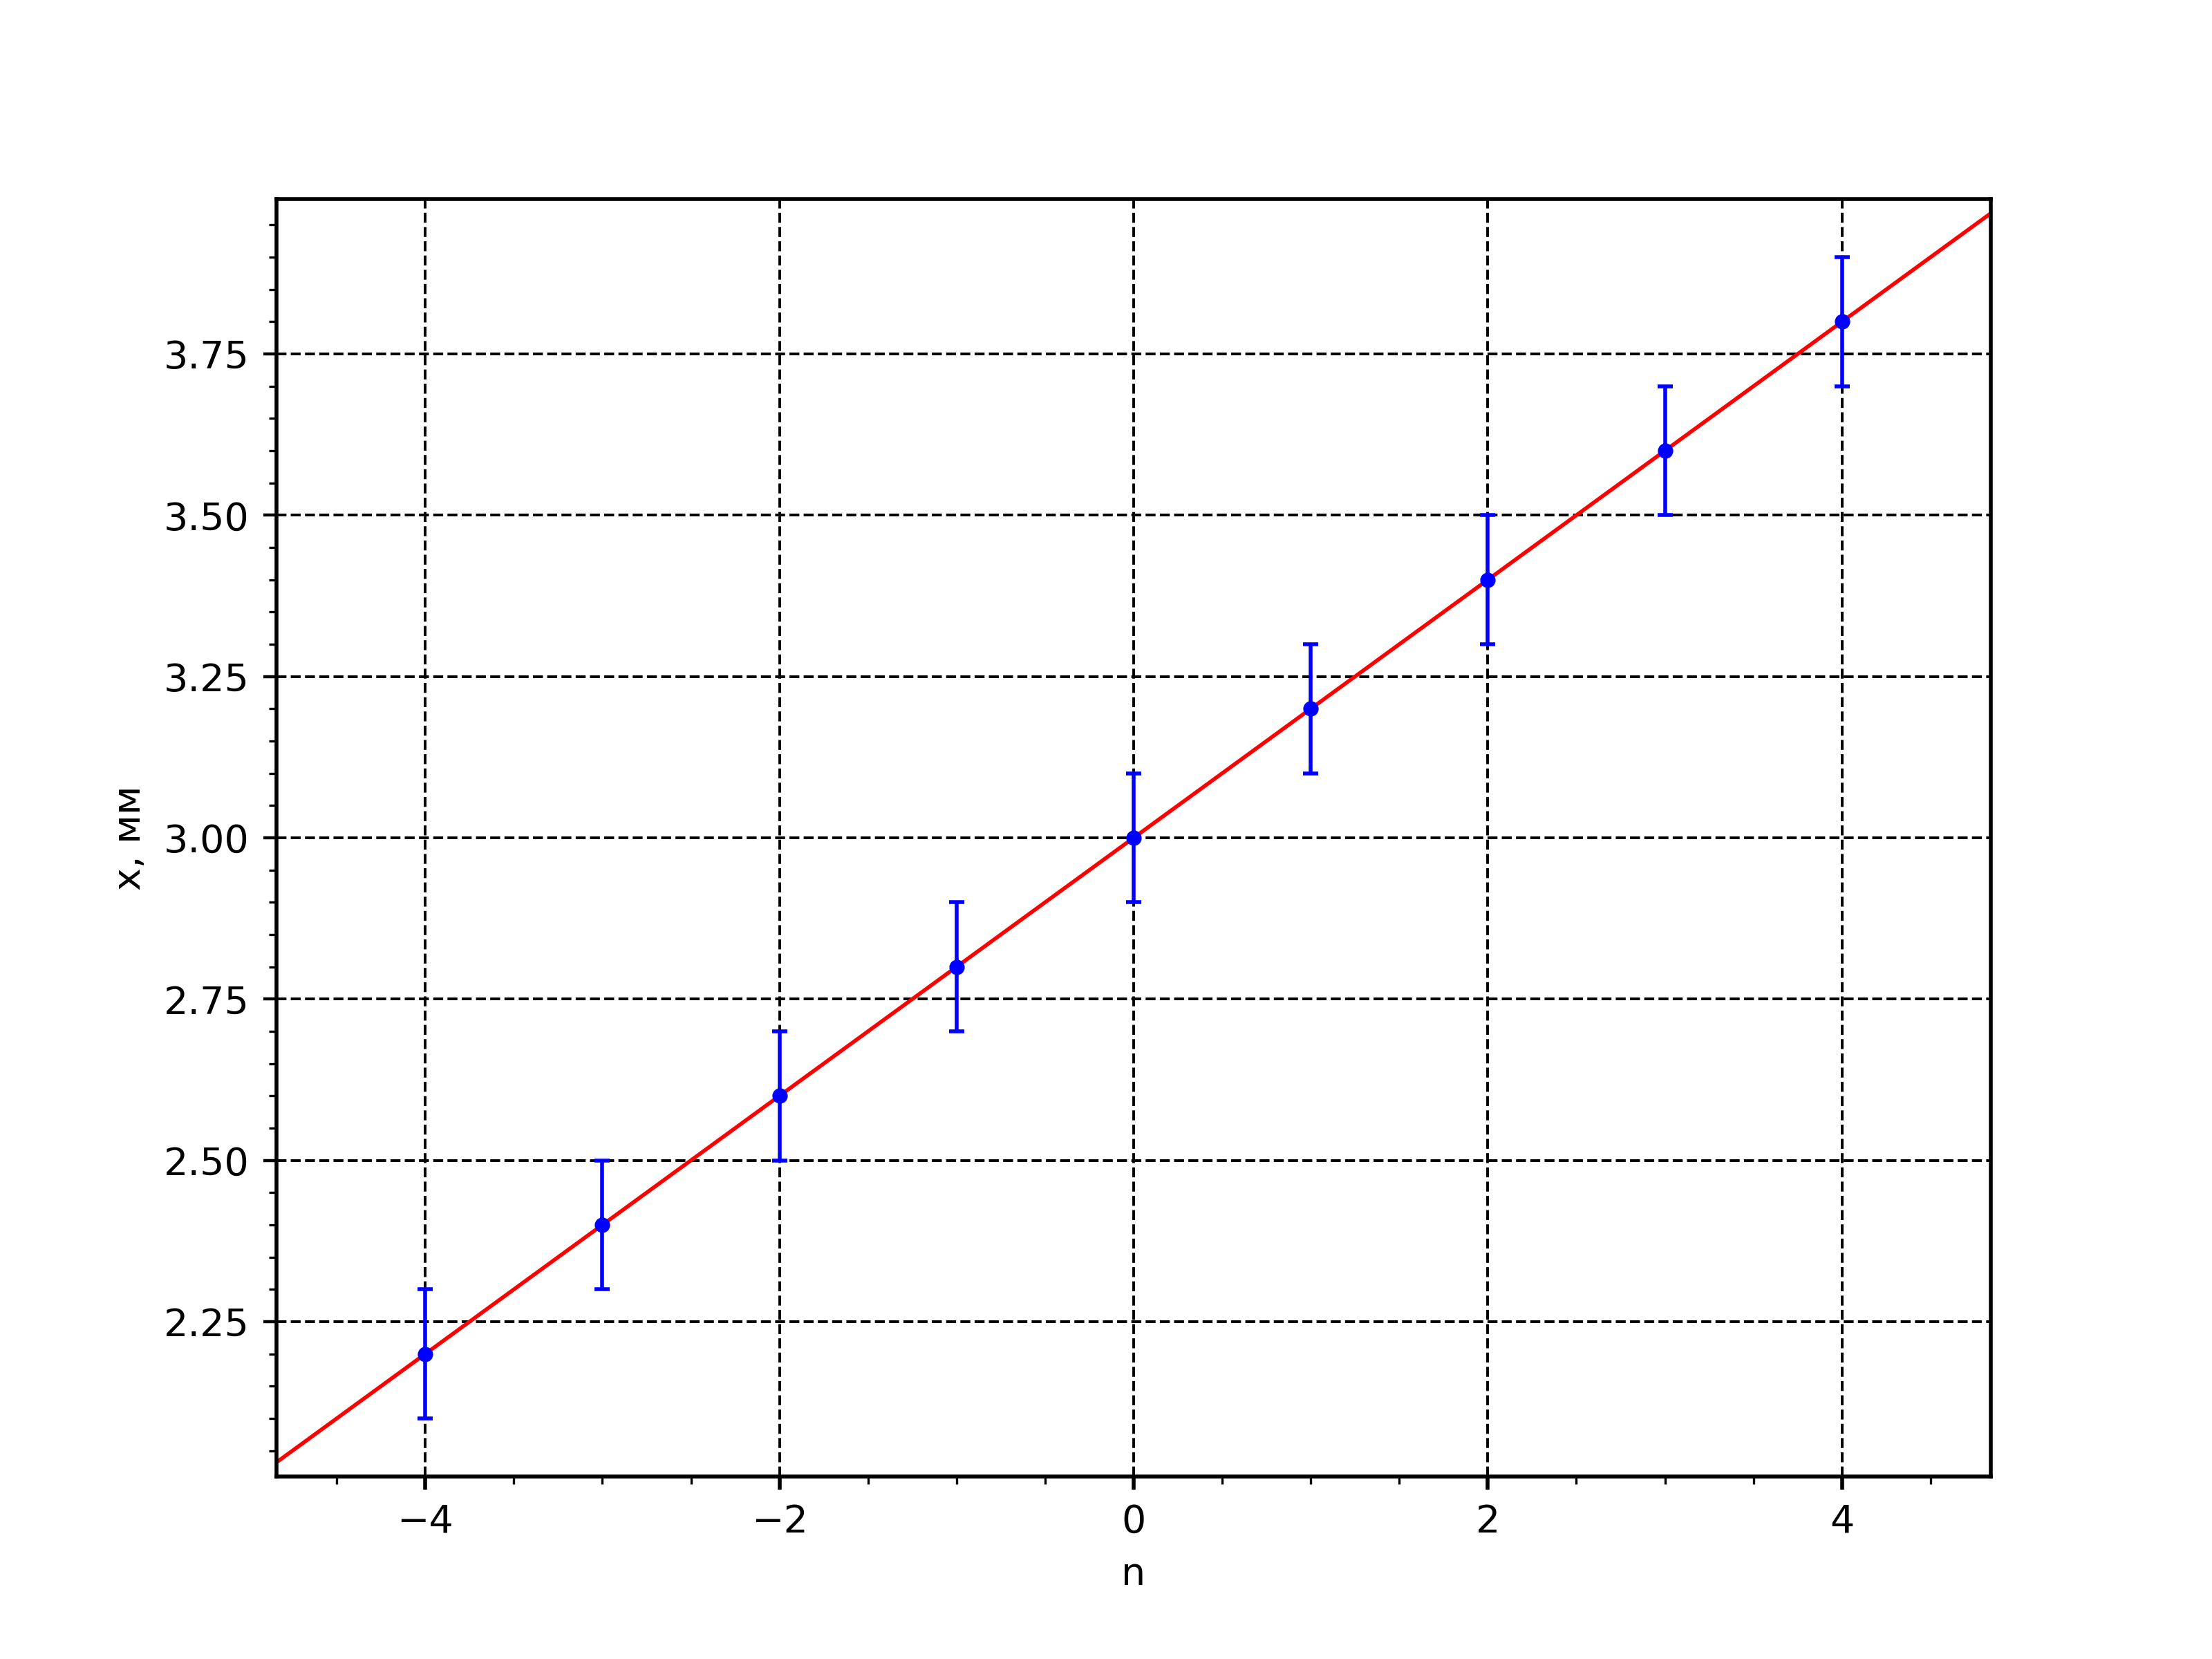
\includegraphics[width=0.8\linewidth]{../img/fuck.png}}
\end{figure}

\[
    k = 0{,}20 \pm 0{,}01\;\text{мм}
\]
\[
    b = \lambda f / k = 0{,}35 \pm 0{,}05 \;\text{мм}
\]

\subsection{Дифракция Фраунгофера на двух щелях}
$n = 12$, $X = 0{,}561 \pm 0{,}001\;\text{мм}$, $\delta x = 0{,}0470 \pm 0{,}0001\;\text{мм}$, $f_{1} = 11{,}0\;\text{см}$, $f_{2} = 12{,}8\;\text{см}$, 

\[
    d = \frac{ \lambda f_{2}}{\delta x} = 1{,}53 \pm 0{,}03\;\text{мм} 
\]
Прямые измерения дают $d = 1{,}55 \pm 0{,}01 \;\text{мм}$, $b_{0} = 0{,}0950 \pm 0{,}0005\;\text{мм}$, $b_{1} = 0{,}1300 \pm 0{,}0005\;\text{мм}$

